
%% Refer to latex document when possible
\documentclass[10pt]{beamer}

%STANDARD PREAMBLE
%https://tex.stackexchange.com/questions/68821/is-it-possible-to-create-a-latex-preamble-header
\usepackage{/Users/mwojno01/Research/Learning/latex_preamble/beamer_preamble}

\title{Why Bayes}
%\subtitle{}

\begin{document}

\maketitle

\begin{frame}{Table of contents}
  \setbeamertemplate{section in toc}[sections numbered] \tableofcontents[hideallsubsections]
\end{frame}

\section{Introduction}
\begin{frame}{Bayesian approaches}

\begin{itemize}
\item Typically contrasted with \textbf{frequentist} approaches
\item Treat parameters as uncertain, data as fixed
\end{itemize}
\end{frame}

%%%%%%%%%%%%%%

\begin{frame}{Bayes' Rule}
\footnotesize

\begin{sblock}{Bayes' Rule}
\[ \underset{posterior}{p(\theta|x)} = \df{ \underset{likelihood}{p(x|\theta)} \quad  \underset{prior}{p(\theta)} }{ \underset{evidence}{p(x)}}  = \dfrac{p(x | \theta) p(\theta)}{\int p(x | \theta) p(\theta) \, d\theta}  \]
\end{sblock}

\begin{sblock}{Posterior}
The posterior distribution is proportional to the prior times the likelihood:
\[p(\theta | x) \propto p(x | \theta) p(\theta)\]

The posterior distribution \textit{is a distribution} over $\theta$.

\end{sblock}

\begin{sblock}{Evidence}
The evidence, or \textit{marginal likelihood}, can be used for model comparison.
\end{sblock}

\end{frame}


\section{Motivations}
\subsection{Avoiding overfitting}

\begin{frame}{Maximum likelihood and overfitting}
Maximum likelihood can have problems with \textbf{over-fitting}. \pause 
\vfill 
The approach can be seen as \textit{over-committing} to a single, fixed parameter value.  \pause 
\vfill 
Bayesian methods can correct this by treating parameters as random variables. 
\end{frame}

\begin{frame}{Bayesian estimation of batting averages}

Let 
\begin{itemize}
\item $x$ be observed data (batting average after $n$ at bats)
\item  $\theta$ be parameters (a player's `true` batting average)
\end{itemize}

	\begin{tikzpicture}
  \node (img)  {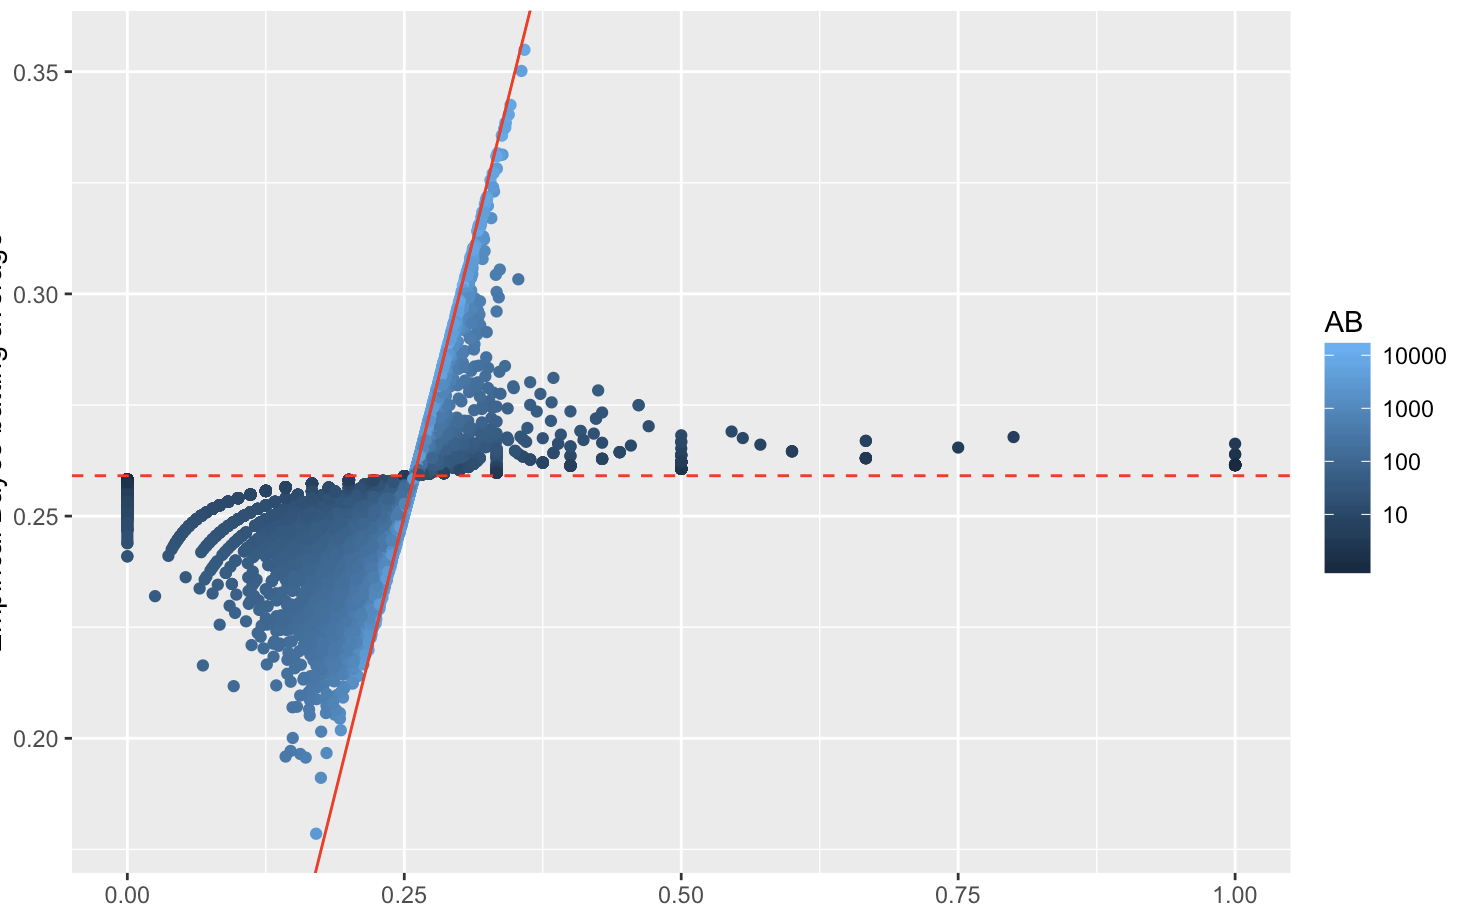
\includegraphics[width=.80\textwidth]{images/batting_averages}} ;
  \node[below=of img, node distance=0cm, yshift=1cm,font=\color{blue}] {Observed data ($x$)};
  \node[left=of img, node distance=0cm, rotate=90, anchor=center,yshift=-0.7cm,font=\color{blue}] {$\E [p (\theta \cond X)]$}; % ($\E_{p(\theta | x)} [\theta]$)};
 \end{tikzpicture}
 
\end{frame}


\begin{frame}{Bayesian Occam's Razor}
\scriptsize

Maximum Likelihood (ML)  solutions tend to overfit.  Bayesian marginalization reduces overfitting.

%\begin{center}
%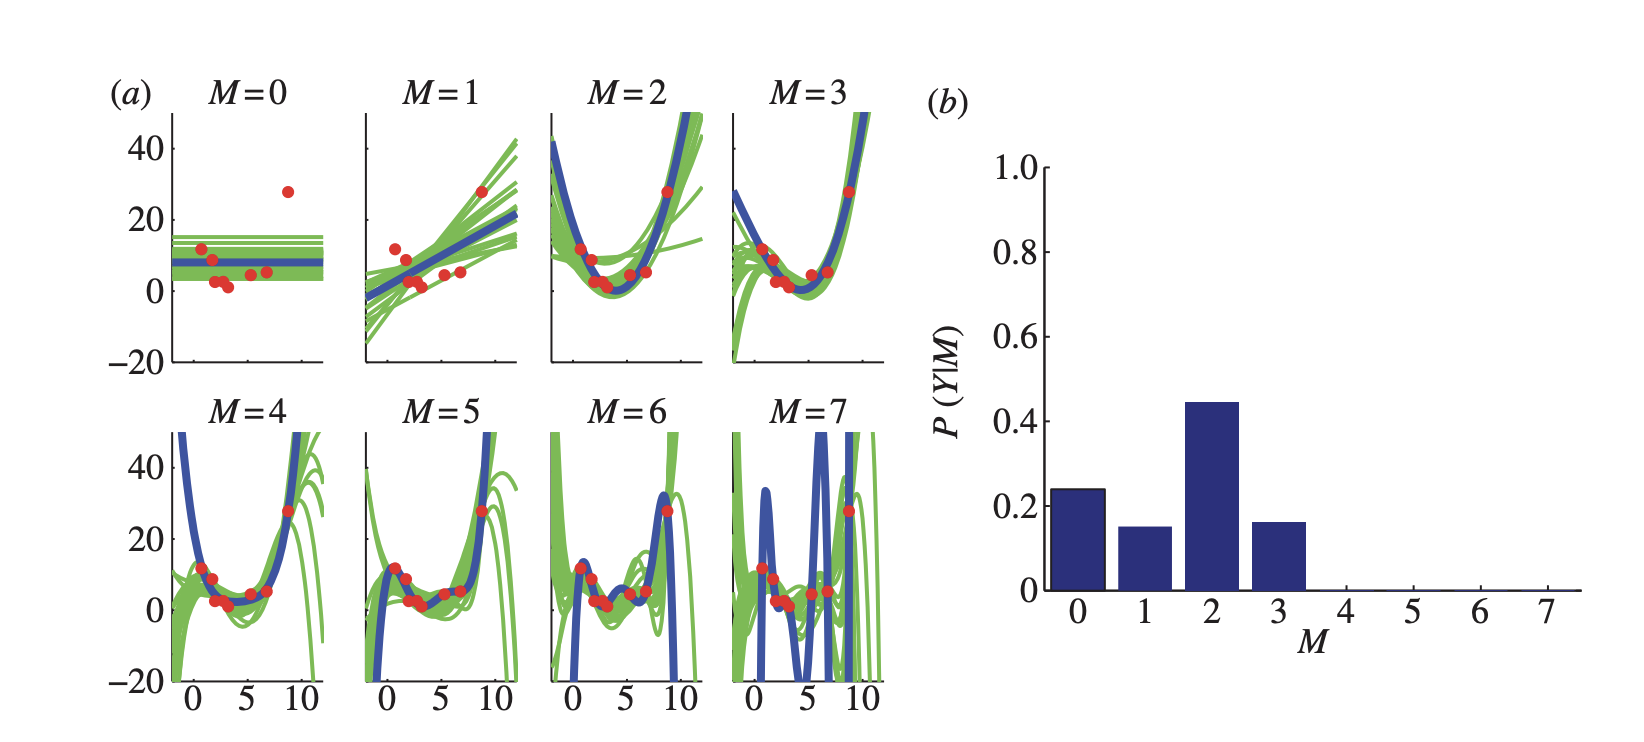
\includegraphics[width=.7\textwidth]{images/occams_razor}
%\end{center}

\begin{minipage}[t]{.47\textwidth}
\begin{center}
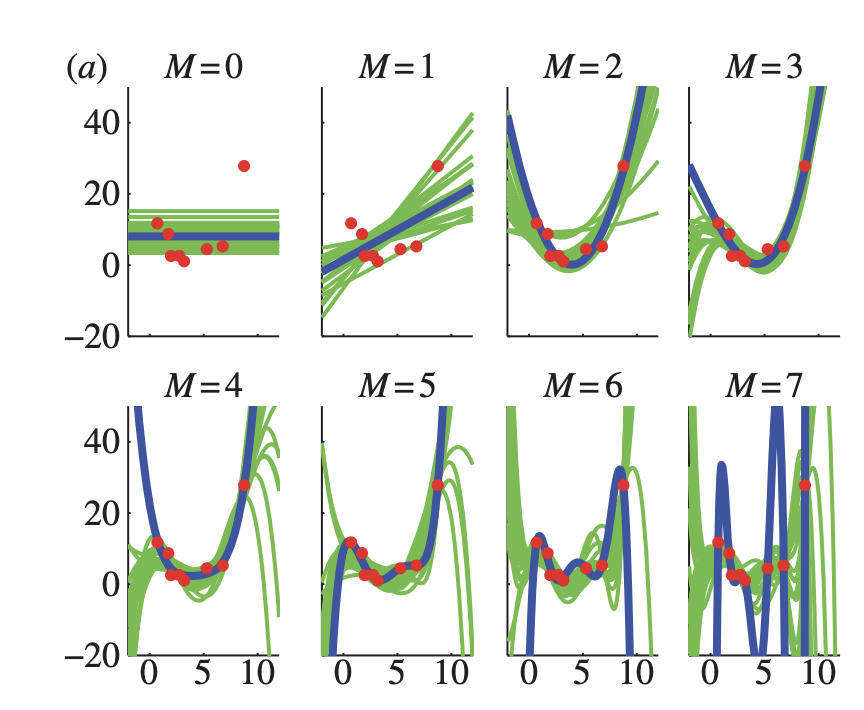
\includegraphics[width=.7\textwidth]{images/occams_razor_a}
\end{center}

Models $y = f(x) + \epsilon$ of  various complexity  \tiny (polynomials of various order, $M$) \scriptsize were fit to 8 data points. 
	\begin{itemize}
	\scriptsize
	\item  Plotted are  \blue{ML} polynomials \tiny (least squares fits to the data under Gaussian noise) \scriptsize and \darkgreen{posterior samples} from a Bayesian model \tiny (which used a Gaussian prior for the coefficients, and an inverse gamma prior on the noise). \scriptsize
	\item The ML estimate can look very different from a typical sample from the posterior!  
	\end{itemize}
\end{minipage}
\hfill
\begin{minipage}[t]{.47\textwidth}
\begin{center}
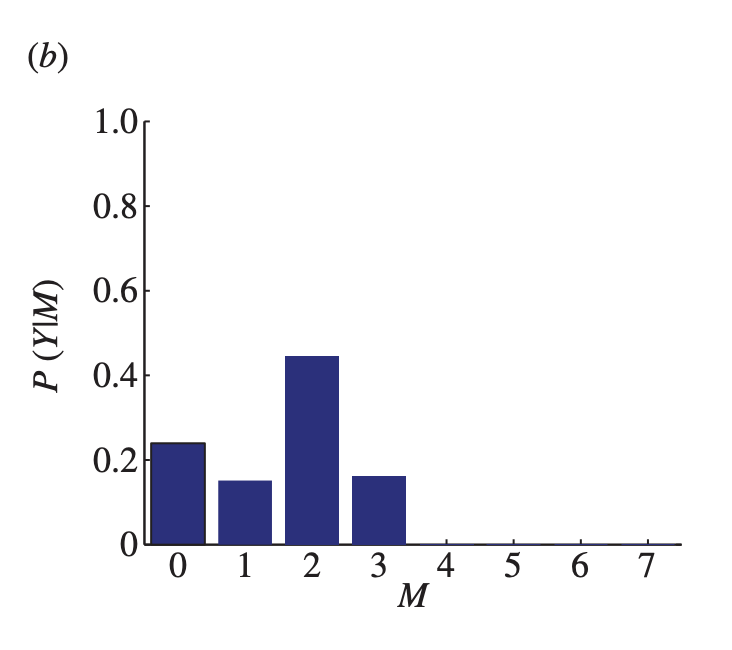
\includegraphics[width=.7\textwidth]{images/occams_razor_b}
\end{center}
The evidence is plotted as a function of model order.  Model orders M=0 to M=3 have considerably higher evidence than other model orders.  We see that Bayesian marginalization has reduced overfitting.  (The maximum likelihood model, the $M=7$ model, fits the data perfectly, but overfits wildly, predicting the function will shoot up or down between neighboring data points.) 
\end{minipage}
\vfill

\hfill \tiny Ghahramani, Z. (2013). Bayesian non-parametrics and the probabilistic approach to modelling. Philosophical Transactions of the Royal Society A: Mathematical, Physical and Engineering Sciences, 371(1984), 20110553.
\end{frame}


\begin{frame}{Bayesian Occam's Razor}
\scriptsize

\begin{center}
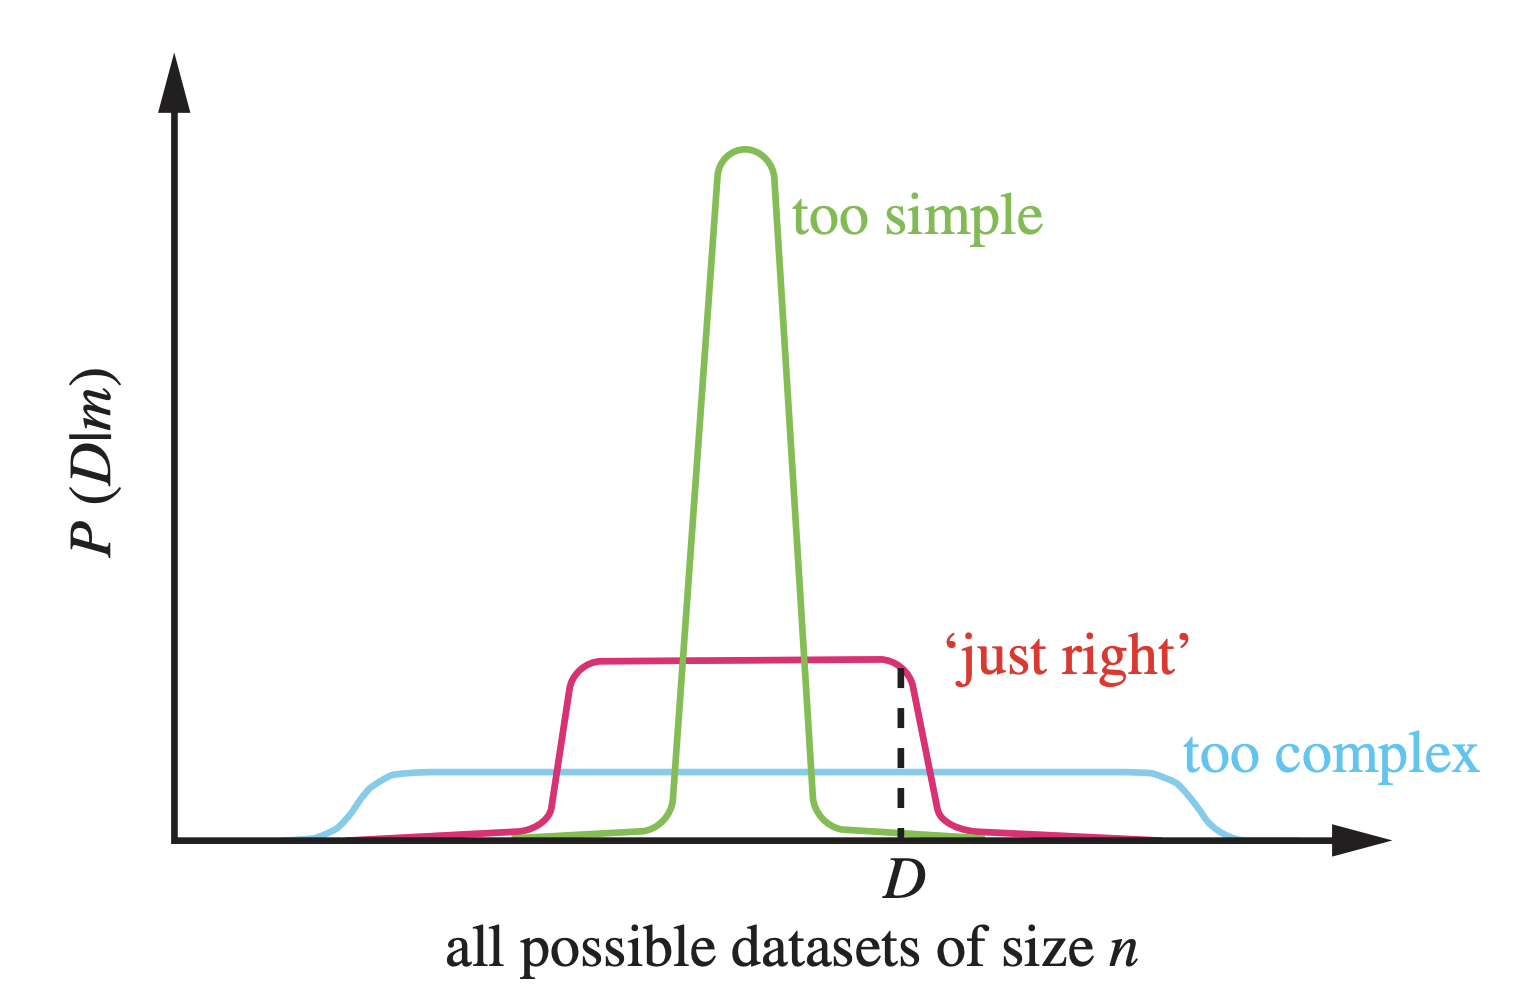
\includegraphics[width=.6\textwidth]{images/auto_occams_razor}
\end{center}
Competing probabilistic models
correspond to alternative distributions over the datasets. Here, we have illustrated three possible models that spread their
probability mass in different ways over these possible datasets. A \textit{complex} model (shown in blue) spreads its mass over many
more possible datasets, whereas a \textit{simple} model (shown in green) concentrates its mass on a smaller fraction of possible data.
Because probabilities have to sum to one, the complex model spreads its mass at the cost of not being able to model simple
datasets as well as a simple model—this normalization is what results in an automatic Occam razor. Given any particular
dataset, here indicated by the dotted line, we can use the marginal likelihood to reject both overly simple models, and overly
complex models. 


\hfill \tiny Ghahramani, Z. (2013). Bayesian non-parametrics and the probabilistic approach to modelling. Philosophical Transactions of the Royal Society A: Mathematical, Physical and Engineering Sciences, 371(1984), 20110553.
\end{frame}


\subsection{Estimating the probability of a rare event}

\begin{frame}{References}

\begin{center}
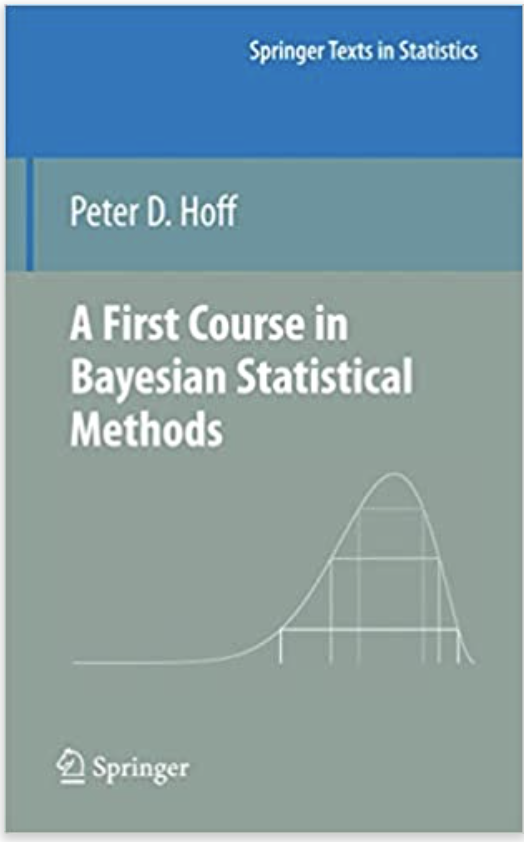
\includegraphics[width=.5\textwidth]{images/hoff_book}
\end{center}

\end{frame}

\begin{frame}{Description of problem}

\begin{itemize}
\item Want to estimate the prevalence of an infectious disease in a small town.
\item The higher the prevalence,  the more public health precautions will be recommended.
\item A small random sample of 20 individuals are checked for infection.
\end{itemize}
\end{frame}

\begin{frame}{Description of problem}

\begin{itemize}
\item \textbf{Parameter} $\theta$,  the fraction of infected individuals in the city.
\item \textbf{Parameter space}:  $\Theta = [0,1]$
\item \textbf{Sample}: $Y$ the number of infected individuals in the sample
\item \textbf{Sample space}: $\mathcal{Y} = \set{0,1,...,20}$
\end{itemize}

\end{frame}

\begin{frame}{Sampling model}

If the value of $\theta$ were known,  a reasonable sampling model for $Y$ would be

\[  Y \cond \theta \sim \Binomial(20, \theta)\]




\begin{figure}
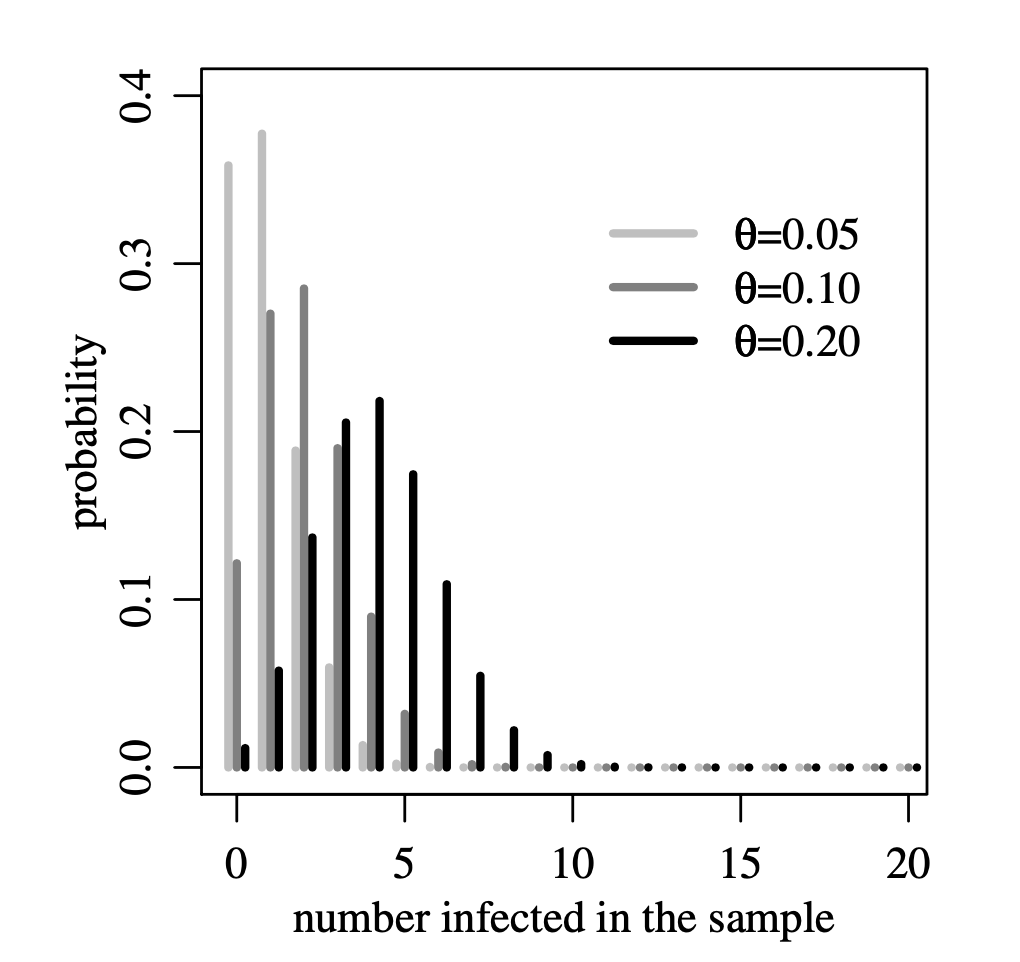
\includegraphics[width=.45\textwidth]{images/binomial_pmf_hoff_example_prob_of_rare_event}
\caption{Binomial$(20,\theta)$ distributons for three values of $\theta$.}
\end{figure}


% SAY:  some implications of various choices of theta.

\end{frame}

\begin{frame}{Prior distribution}
Other studies from various parts of the country indicate that the infection rate in comparable cities range from about 0.05 to 0.20, with an average prevalence of 0.10.

\pause 

This suggests we use a prior distribution $p(\theta)$ that assigns a substantial amount of probability to the interval $(0.05, 0.20)$.
\pause 

\begin{center}
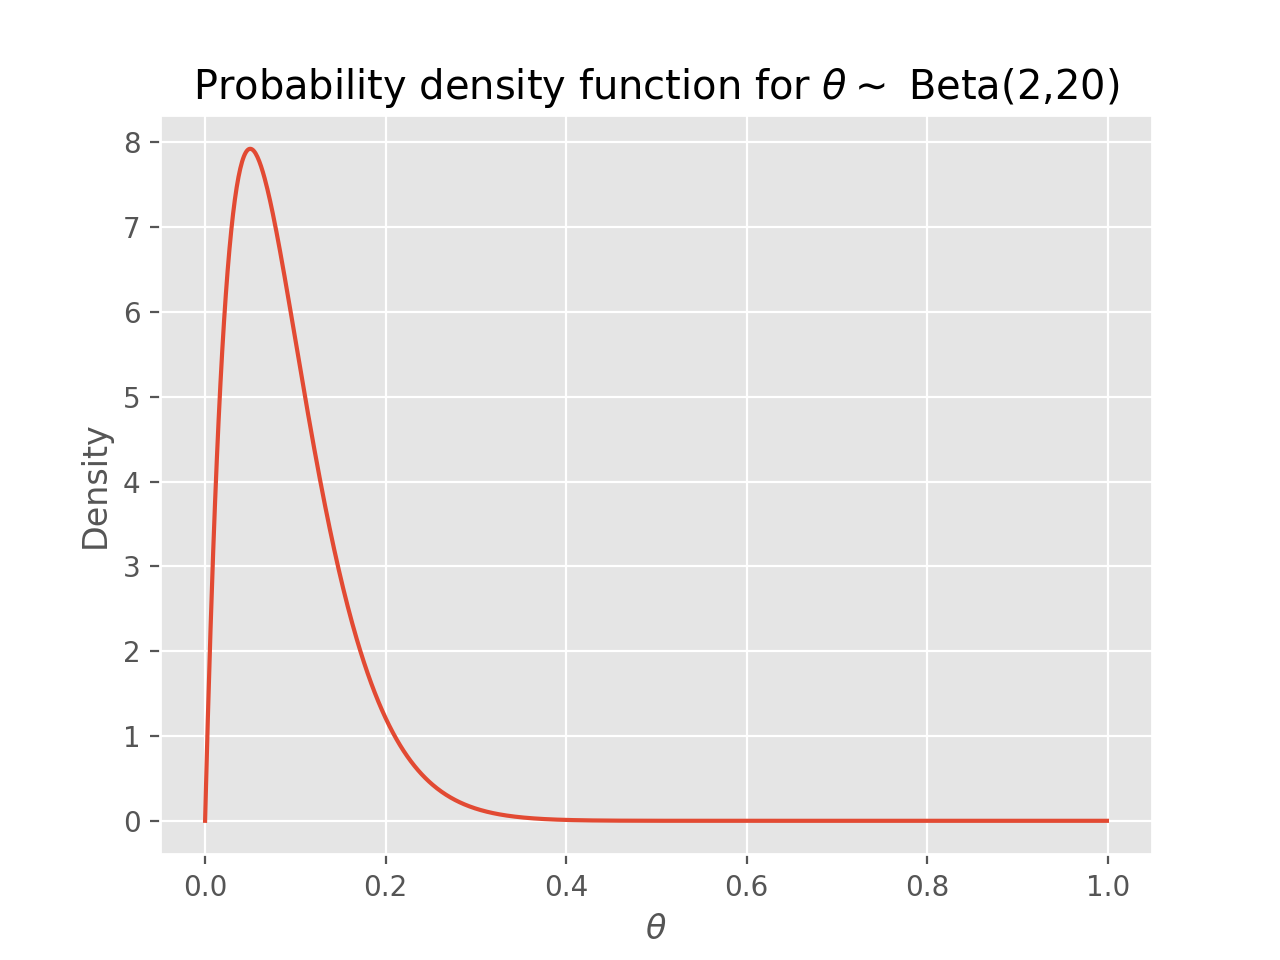
\includegraphics[width=.45\textwidth]{images/beta_pdf}
\end{center}

We can encode this prior information using
\[  \theta \sim \Beta(2,20) \] 

% DISCUSS: How the Beta captures the prior knowledge

\end{frame}


\begin{frame}{From prior to posterior}

\begin{center}
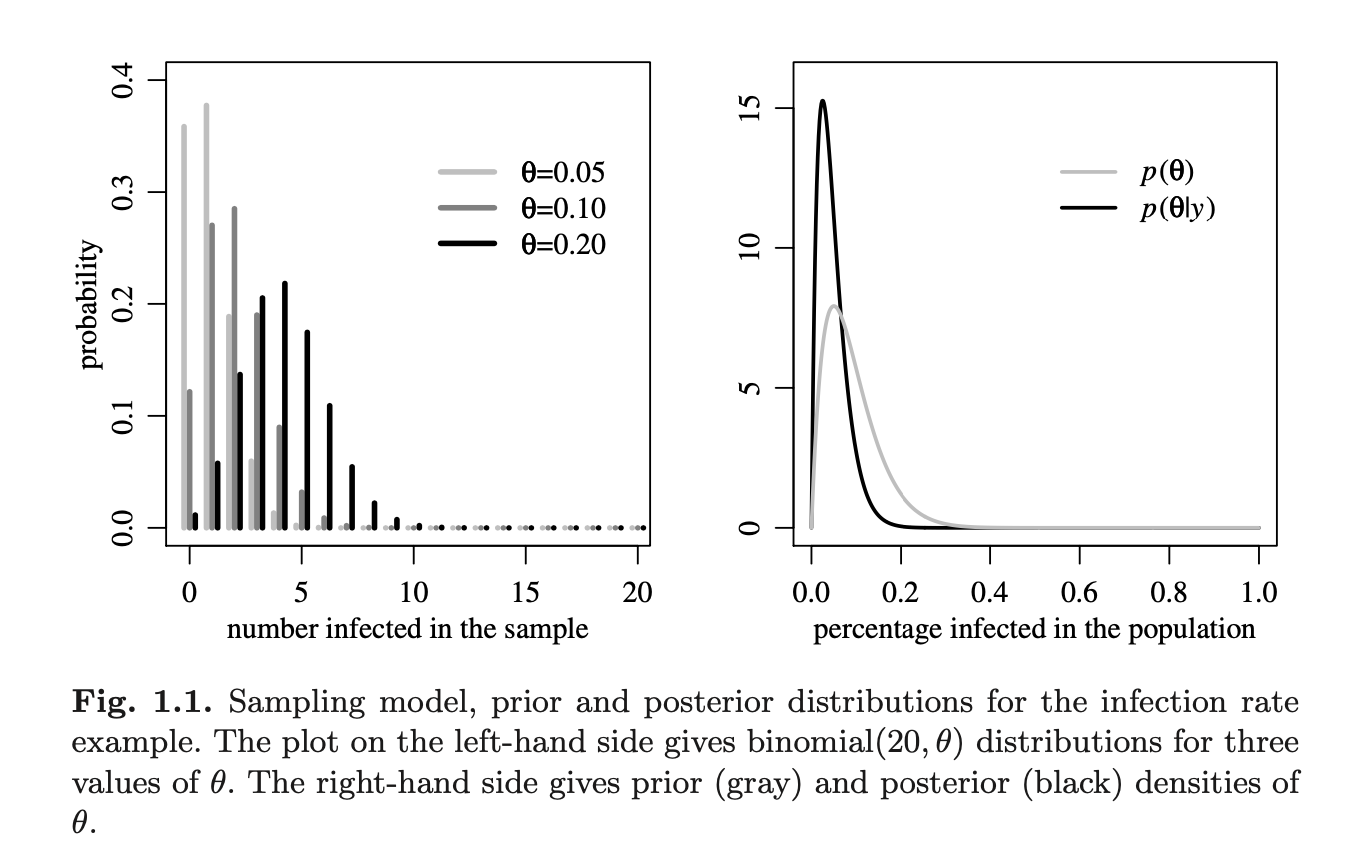
\includegraphics[width=.75\textwidth]{images/hoff_fig1dot1_prior_posterior_shift}
\end{center}

\scriptsize
\begin{minipage}{.45\textwidth}

\begin{align*}
\textbf{Prior} & \\
\theta  \sim  \Beta(2,20)   &\\ 
\E[\theta]  = 0.09 &\\
\text{mode}[\theta] =0.05 &\\
P(\theta < 0.10) = 0.64 &\\
P(0.05 < \theta < 0.20) = 0.66&  \\
\end{align*}

\end{minipage} \hfill
\begin{minipage}{.45\textwidth}

\begin{align*}
\textbf{Posterior} & \\
\theta \cond \set{Y=0}  \sim  \Beta(4,20)  &  \\ 
\E[\theta \cond \set{Y=0}  ] = 0.048& \\
\text{mode}[\theta \cond \set{Y=0}  ] =0.025& \\
P(\theta < 0.10 \cond \set{Y=0} ) = 0.93 &\\
\end{align*}

\end{minipage}


\end{frame}


\begin{frame}{Sensitivity analysis}
Suppose we consider beliefs represented by $\Beta(a,b)$ distributions for $(a,b)$ other than $(2,20)$.   

If $\theta \sim \Beta(a,b)$,  then $\theta \cond Y=y \sim \Beta(a+y,  b+n-y)$.  

The posterior expectation is

\begin{align*}
\E[\theta \cond Y=y] &= \df{a+y}{a+b+n} \\
&= \df{n}{a+b+n} \df{y}{n} + \df{a+b}{a+b+n} \df{a}{a+b} \\
& = \df{n}{w+n}  \bar{y} + \df{w}{w+n} \theta_0 \\
\end{align*}
where $\theta_0 = a/(a+b)$ is the prior expectation of $\theta$ and $w=a+b$.
\pause 

So the posterior expectation is a compromise between the prior expectation $\theta_0$ and sample mean $\bar{y}$.  The weights on each depend on the sample size,  $n$,  and our prior confidence in this guess,  $w$. 
\end{frame}

\begin{frame}{Sensitivity analysis}

If someone provides us with a prior guess $\theta_0$ and degree of confidence $w$,  then we can approximate their prior beliefs about $\theta$ with
\[ Beta \bigg(  a = w \theta_0 ,  \quad  b= w (1-\theta_0) \bigg) \]
And their posterior beliefs are represented with 
\[ Beta \bigg(  a = w \theta_0 + y  ,  \quad  b= w (1-\theta_0) + n-y \bigg) \] 
\pause 
We can compute such a posterior distribution for a wide range of $\theta_0$ and $w$ values to perform a \textit{sensitivity analysis},  an exploration of how posterior information is affected by differences in prior opinion.

% SAY: We might be interested in the changes in the opinions of a wide range of public health officials with heterogeneous prior opinions.   (One might think the town has fewer infections than similar towns,  but not be very confident about it.   Another might think the town has more infections than simialr towns,  and be super confident about it.)

\end{frame}

\begin{frame}{Sensitivity analysis}
\begin{center}
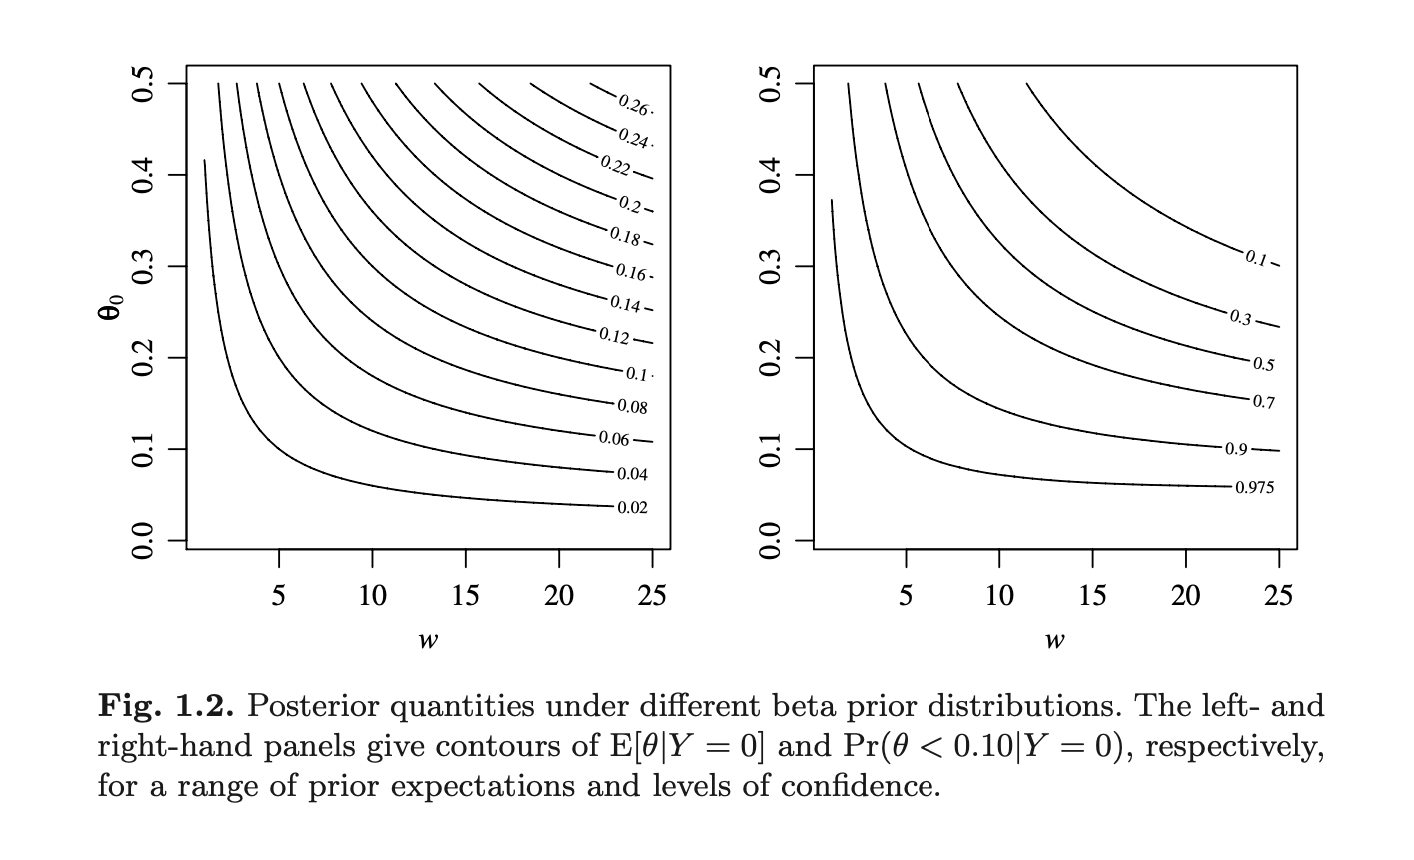
\includegraphics[width=.8\textwidth]{images/hoff_fig1dot2_sensitivity_analysis}
\end{center}

The second plot may be of use if,  e.g.,  city officials would like to recommend a vaccine to the general public unless they were reasonably sure the current infection rate was less than 0.10.  

\pause  \scriptsize
A high degree of certainty (say $97.5\%$) is only achieved by people who already thought the infection rate was lower than the average of other cities.

\end{frame}

\begin{frame}{Comparison to non-Bayesian methods}
A 95$\%$ confidence interval for population proportion $\theta$ is the \textit{Wald interval}, 
given by

\[ \bar{y} \pm 1.96 \sqrt{\bar{y} (1 - \bar{y}) / n} \]

\pause 


The interval has \textit{correct asymptotic frequentist coverage},  meaning that if $n$ is large,  then with probability approximately equal to 95\%,  $Y$ will take on a value $y$ such that the above interval contains $\theta$.

\pause 

For our sample in which $\bar{y} = 0$,  the Wald confidence interval comes out to be just a single point: 0.

\pause 

In fact,  the 99.99\% Wald interval also comes out to be zero.

\end{frame}

\begin{frame}{Comparison to non-Bayesian methods}

People have suggested alternatives to avoid this type of behavior.  \pause 

The ``adjusted" Wald interval suggested by Agresti and Coull (1998) is given by

\begin{align*}
\widehat{\theta} & \pm \sqrt{\widehat{\theta} (1 - \widehat{\theta}) / n},  \quad \text{where} \\
\widehat{\theta}  &= \df{n}{n+4} \bar{y} + \df{4}{n+4} \df{1}{2}
\end{align*}

\pause 
While not motivated as such,  the interval is clearly related to Bayesian inference:  $\widehat{\theta}$ is equivalent to the posterior mean for $\theta$ under a $\Beta(2,2)$ prior,  which represents weak prior information centered around $\theta = 1/2$.

\end{frame}

\begin{frame}{Comparison to non-Bayesian methods}

Compared to the post-hoc ``adjustment" approach,  the Bayesian formalism provides

\begin{itemize}
\item Reasonable conclusions which fall naturally out of the framework
\item Flexibility to other choice of priors than $\Beta(2,2)$
\item Sensitivity analysis to consider the sets of conclusions that would be reached by people with different priors. 
\item Simultaneous access to various functionals of the posterior -- not just $\E[\theta \cond Y= y]$ but also $\P [\theta < 0.10 \cond Y=0]$.
\end{itemize}

\end{frame}

\section{Conclusion}

\begin{frame}{Summary}
\textit{What are some advantages of the Bayesian approach?} \pause 
\begin{itemize}
\item Exploits prior knowledge {\tiny (previous results, reasonable values of data, etc.)} \pause 
\item Automatic complexity control \pause 
\item Immediate access to many inferential quantities of inference \pause 
\item Natural (and more flexible) solutions to frequentist problems:  {\tiny (adjustments to confidence intervals, regularization, etc.) }  \pause 
\item Can be easier in practice to extend to more complex models 
\end{itemize}
	
\end{frame}

\begin{frame}{Extensions: Hierarchical models}

\begin{itemize}
\item Hierarchical models use ``surrounding data" as a prior in a more formal way.   
\item In Hoff's disease prevalence example,  we constructed our beta prior manually,  by taking a couple of basic facts about similar towns and then converting that into beta parameters.    
\item A hierarchical model could let the prior expectation be tied more exactly to those surrounding towns.   We can automatically set the strength of the prior expectation according to the relative uncertainty within and between towns,  and to automatically adapt as data rolls in. 
\item Hierarchical regressions allow the prior expectation to be more strongly influenced by towns that are similar w.r.t. \text{relevant} characteristics,  such as size,  SES,  etc
\end{itemize}
\end{frame}

\begin{frame}{Utility for large datasets}


\begin{itemize}
\item Still useful for larger models
\vfill 
\item Especially complex models -- what really matters is the information we get about a given parameter.
\vfill 
\begin{quotation}
A big dataset is just a bunch of small datasets	
\end{quotation}
\vfill 
\item Example: biometric profiling.  {\tiny (A given bigram may be rare to type, but in the end, you're typing \textit{some} rare bigram a high percentage of the time!) }
\end{itemize}

% TODO OR DISCUSS: Still useful for larger models.      Especially complex models - what really matters it the information we get about a given parameter.  Mention the yalnce biometric profiling.   A given bigram may be rare to type,  but in the end you're typing some rare bigram a high percentage of the time!  Mike Hughes mentioned Andrew Gelman's blog post " a big dataset is just a bunch of small datasets".   
\end{frame}

\end{document}



